\begin{figure} \begin{center}\centering
        \caption{ABC Birth Cohort: Total Annual Earnings, Females Age 30}
        \label{female_earn_decile_abc}\vspace{0.2cm}
         \subfloat[How the Black Disadvantaged Fit into the Black Distribution at Age 30, by decile]{
                \scalebox{0.75}{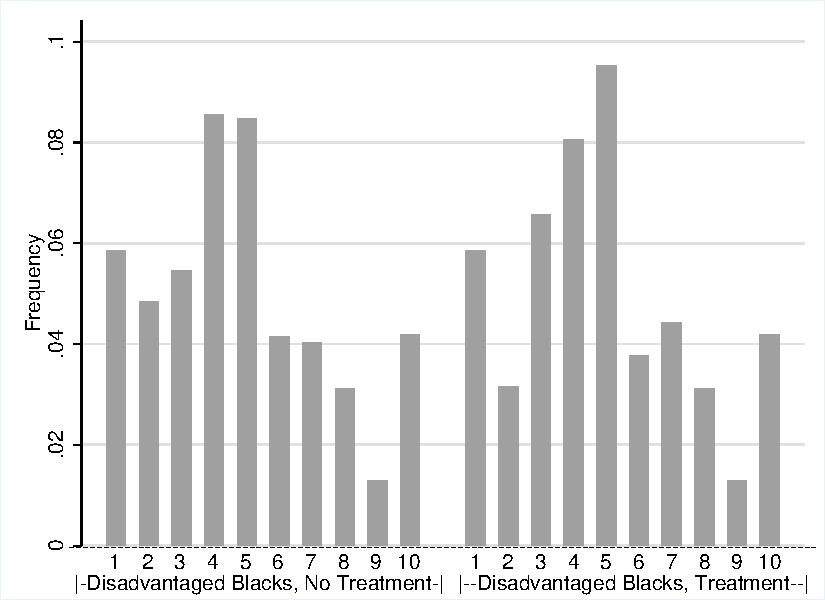
\includegraphics{female3_abc}}} \\
         \subfloat[How the Black Fit into the White Distribution at Age 30, by decile]{
                \scalebox{0.75}{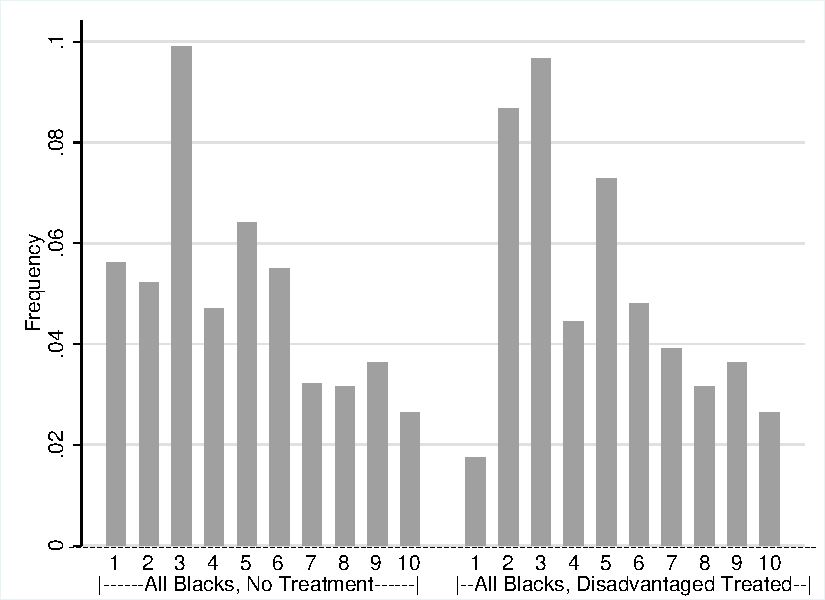
\includegraphics{female4_abc}}} \\     
\end{center}
{\scriptsize {\bfseries Notes: } \raggedright Earnings are three year averages centered at age 30. The black disadvantaged group satisfies the ABC eligibility criteria. The black non-disadvantaged do not satisfy this criteria. Black and white are representative of the cohort born between 1972 and 1977. The left hand side plots consider the cases of the No Action Scenario (Scenario 1): the ABC Program does not influence adult outcomes. The right hand side plots consider cases of the Counter-factual Scenario (Scenario 2): we apply the gender-specific treatment effects of the ABC Program to the disadvantaged black population. We use the treatment effects calculated by \citet{Frances_2013_EJ}.
}
\end{figure}

\begin{figure} \begin{center}\centering
        \caption{ABC Birth Cohort: Total Annual Earnings, Males Age 30}
        \label{male_earn_decile_abc}\vspace{0.2cm}        
         \subfloat[How the Black Disadvantaged Fit into the Black Distribution at Age 30, by decile]{
                \scalebox{0.75}{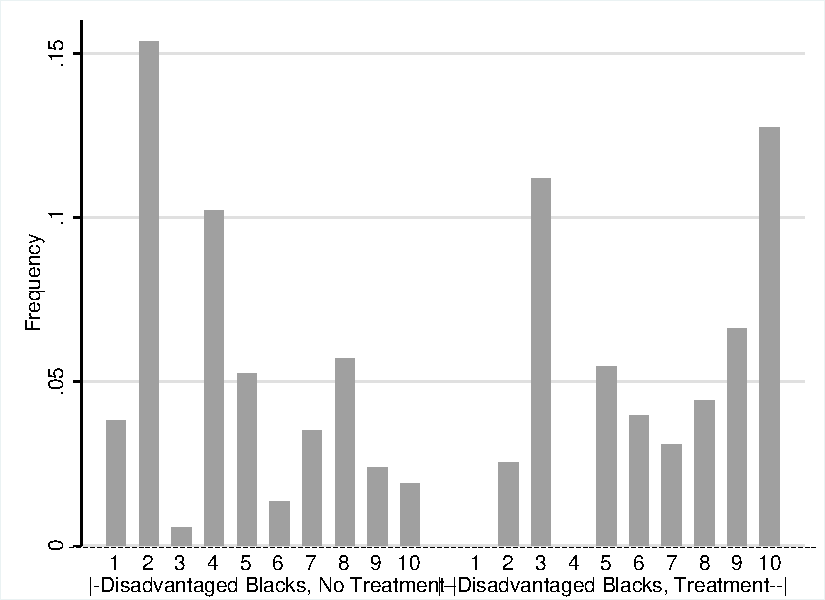
\includegraphics{male3_abc}}} \\
         \subfloat[How the Black Fit into the White Distribution at Age 30, by decile]{
                \scalebox{0.75}{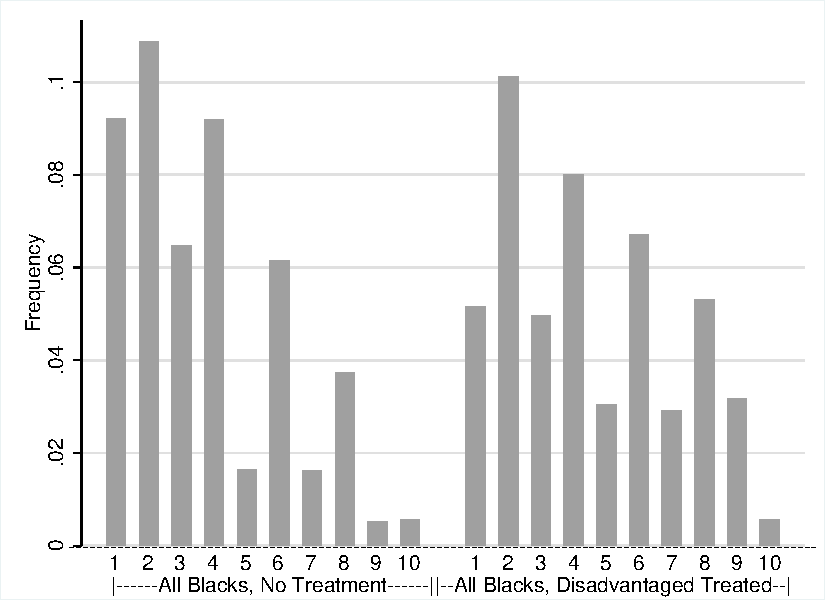
\includegraphics{male4_abc}}} \\
\end{center}
{\scriptsize {\bfseries Notes: } \raggedright Earnings are three year averages centered at age 30. The black disadvantaged group satisfies the ABC eligibility criteria. The black non-disadvantaged do not satisfy this criteria. Black and white are representative of the cohort born between 1972 and 1977. The left hand side plots consider the cases of the No Action Scenario (Scenario 1): the ABC Program does not influence adult outcomes. The right hand side plots consider cases of the Counter-factual Scenario (Scenario 2): we apply the gender-specific treatment effects of the ABC Program to the disadvantaged black population. We use the treatment effects calculated by \citet{Frances_2013_EJ}. 
}
\end{figure}


